\documentclass[aspectratio=169]{beamer}

% -------------------------
% 1.  PACKAGES & THEME
% -------------------------
\usepackage[english]{babel}
\usepackage{fontawesome5}
\usepackage{tikz}
\usetikzlibrary{positioning,calc,shapes.geometric,backgrounds,patterns}
\usepackage{FiraSans}
\usepackage{FiraMono}
\usepackage{graphicx}
\usepackage{hyperref}
\usepackage{booktabs}
\usepackage{pgf-pie}
\usepackage{xcolor}

% Theme & colors - CONSISTENT PALETTE
\usetheme{metropolis}

% Primary brand colors
\definecolor{primary}{HTML}{FF6600}      % Orange (main brand color)
\definecolor{secondary}{HTML}{9945FF}    % Purple (secondary brand)
\definecolor{accent}{HTML}{14F195}       % Green (accent for highlights)

% Background colors
\definecolor{darkbg}{HTML}{0B0F1A}       % Dark background
\definecolor{midbg}{HTML}{1A1F2E}        % Medium background
\definecolor{lightbg}{HTML}{2D3748}      % Light background/panels

% Text and UI colors
\definecolor{textprimary}{HTML}{FFFFFF}  % Primary text (white)
\definecolor{textsecondary}{HTML}{B8BCC8} % Secondary text (light gray)
\definecolor{highlight}{HTML}{FFD700}     % Gold for special emphasis

% Semantic colors
\definecolor{success}{HTML}{14F195}      % Success/positive (green)
\definecolor{warning}{HTML}{FFD700}      % Warning/important (gold)
\definecolor{info}{HTML}{00D1FF}         % Info/neutral (cyan)

\setbeamercolor{background canvas}{bg=darkbg}
\setbeamercolor{normal text}{fg=textprimary}
\setbeamercolor{alerted text}{fg=primary}
\setbeamercolor{example text}{fg=secondary}
\setbeamercolor{frametitle}{fg=textprimary,bg=darkbg}
\setbeamercolor{title}{fg=textprimary}

\setbeamerfont{title}{size=\Huge,series=\bfseries}
\setbeamerfont{subtitle}{size=\Large}
\setbeamerfont{author}{size=\normalsize}
\setbeamerfont{date}{size=\small}
\setbeamerfont{frametitle}{size=\Large,series=\bfseries}

% No nav symbols, clean footer with slide numbers
\setbeamertemplate{navigation symbols}{}
\setbeamertemplate{footline}{%
  \hfill%
  \usebeamerfont{page number in head/foot}%
  \color{textsecondary}\insertframenumber\,/\,\inserttotalframenumber\kern1em\vskip2pt%
}

% Custom itemize bullets
\setbeamertemplate{itemize items}[circle]
\setbeamercolor{itemize item}{fg=primary}
\setbeamercolor{itemize subitem}{fg=secondary}

% -------------------------
% 2.  TITLE SLIDE
% -------------------------
\title{FUN GERBIL}

\begin{document}

% -------------------------------------------------
\begin{frame}[plain]
  
\begin{tikzpicture}[remember picture,overlay]
    % Epic gradient background with overlays
    \fill[darkbg] (current page.south west) rectangle (current page.north east);
    \fill[primary,opacity=0.15] (current page.south west) -- 
          (current page.north west) -- 
          ([yshift=-3cm]current page.north east) -- 
          ([yshift=2cm]current page.south east) -- cycle;
    \fill[secondary,opacity=0.1] ([xshift=3cm]current page.south west) -- 
          ([xshift=-2cm]current page.north west) -- 
          (current page.north east) -- 
          (current page.south east) -- cycle;
    
    % Animated circuit pattern overlay
    \foreach \x in {0,1,2,...,20} {
      \foreach \y in {0,1,2,...,12} {
        \fill[info,opacity=0.03] ([shift={(0.8*\x cm, 0.8*\y cm)}]current page.south west) circle (0.5pt);
      }
    }
    
    % Main title content with epic styling
    \node[align=center] at (current page.center){
      % Main title - MASSIVE and bold with glow effect
      {\fontsize{72}{80}\selectfont\color{primary!40}\textbf{FUN GERBIL}}\\[-4.6em]
      {\fontsize{72}{80}\selectfont\color{textprimary}\textbf{FUN GERBIL}}\\[1.2em]
      
      % Subtitle - clean and simple
      {\fontsize{42}{50}\selectfont\color{primary}\textbf{onboarding Monero}}
    };
    
    % Corner decorative elements
    \fill[highlight,opacity=0.8] (current page.south west) -- ++(2,0) -- ++(0,0.1) -- ++(-2,0) -- cycle;
    \fill[info,opacity=0.8] (current page.north east) -- ++(-2,0) -- ++(0,-0.1) -- ++(2,0) -- cycle;
    
  \end{tikzpicture}
\end{frame}

% -------------------------------------------------
\begin{frame}[t]{\color{textprimary}\textbf{Fun Gerbil: Privacy for Solana, DeFi for Monero}}

  \vspace{0.5em}
  
  \begin{columns}[T]
    % Left column - Solana Problems
    \begin{column}{0.48\textwidth}
      \centering
      \begin{tikzpicture}
        % Background box for Solana
        \fill[secondary,opacity=0.15,rounded corners=15pt] (-3.5,-4.2) rectangle (3.5,2.2);
        
        % Solana Logo
        \node at (0,1.5) {\includegraphics[height=1.2cm]{solana-logo.png}};
        
        % Title
        \node[text=secondary,font=\Large\bfseries] at (0,0.5) {Solana};
        
        % Two problems
        \node[text=accent,font=\large] at (-2.5,-1.3) {\faEye};
        \node[text=textprimary,font=\Large\bfseries,align=left,text width=4.5cm] at (0.3,-1.3) {Public Account\\Balances};
        
        \node[text=accent,font=\large] at (-2.5,-2.8) {\faUserSecret};
        \node[text=textprimary,font=\Large\bfseries,align=left,text width=4.5cm] at (0.3,-2.8) {Every Transaction\\Visible};
      \end{tikzpicture}
    \end{column}
    
    % Right column - Monero Problems
    \begin{column}{0.48\textwidth}
      \centering
      \begin{tikzpicture}
        % Background box for Monero
        \fill[primary,opacity=0.15,rounded corners=15pt] (-3.5,-4.2) rectangle (3.5,2.2);
        
        % Monero Logo
        \node at (0,1.5) {\includegraphics[height=1.2cm]{monero-logo.png}};
        
        % Title
        \node[text=primary,font=\Large\bfseries] at (0,0.5) {Monero};
        
        % Two problems
        \node[text=accent,font=\large] at (-2.5,-1.3) {\faCode};
        \node[text=textprimary,font=\Large\bfseries,align=left,text width=4.5cm] at (0.3,-1.3) {No Native \\Programmability};
        
        \node[text=accent,font=\large] at (-2.5,-2.8) {\faBan};
        \node[text=textprimary,font=\Large\bfseries,align=left,text width=4.5cm] at (0.3,-2.8) {Facing Exchange\\Delistings};
      \end{tikzpicture}
    \end{column}
  \end{columns}

\end{frame}

% -------------------------------------------------
\begin{frame}[t]{\color{textprimary}\textbf{Fun Gerbil: Past Barriers to Entry are Gone}}
  \begin{tikzpicture}[remember picture,overlay]
    \fill[primary,opacity=0.05] (current page.south west) rectangle (current page.north east);
  \end{tikzpicture}
  
  \centering
  
  \begin{tikzpicture}
    % Six barriers in 2 rows of 3 - BIGGER
    % Row 1 - 3 items
    \begin{scope}[shift={(-4.5,1.5)}]
      \fill[midbg,rounded corners=12pt] (-2.2,-1.3) rectangle (2.2,1.3);
      \node[text=primary,font=\Large] at (0,0.6) {\faChartLine};
      \node[text=textprimary,font=\normalsize\bfseries,align=center,text width=4cm] at (0,-0.4) {DeFi Was Too Small\\vs CeFi};
    \end{scope}
    
    \begin{scope}[shift={(0,1.5)}]
      \fill[midbg,rounded corners=12pt] (-2.2,-1.3) rectangle (2.2,1.3);
      \node[text=success,font=\Large] at (0,0.6) {\faCheckCircle};
      \node[text=textprimary,font=\normalsize\bfseries,align=center,text width=4cm] at (0,-0.4) {CEXs Supported\\Monero};
    \end{scope}
    
    \begin{scope}[shift={(4.5,1.5)}]
      \fill[midbg,rounded corners=12pt] (-2.2,-1.3) rectangle (2.2,1.3);
      \node[text=info,font=\Large] at (0,0.6) {\faLink};
      \node[text=textprimary,font=\normalsize\bfseries,align=center,text width=4cm] at (0,-0.4) {FCMP Enables\\Transaction Chaining};
    \end{scope}
    
    % Row 2 - 3 items
    \begin{scope}[shift={(-4.5,-1.5)}]
      \fill[midbg,rounded corners=12pt] (-2.2,-1.3) rectangle (2.2,1.3);
      \node[text=warning,font=\Large] at (0,0.6) {\faDollarSign};
      \node[text=textprimary,font=\normalsize\bfseries,align=center,text width=4cm] at (0,-0.4) {No Centralized Grant\\Foundation Funding};
    \end{scope}
    
    \begin{scope}[shift={(0,-1.5)}]
      \fill[midbg,rounded corners=12pt] (-2.2,-1.3) rectangle (2.2,1.3);
      \node[text=secondary,font=\Large] at (0,0.6) {\faBalanceScale};
      \node[text=textprimary,font=\normalsize\bfseries,align=center,text width=4cm] at (0,-0.4) {Regulatory Fallout};
    \end{scope}
    
    \begin{scope}[shift={(4.5,-1.5)}]
      \fill[midbg,rounded corners=12pt] (-2.2,-1.3) rectangle (2.2,1.3);
      \node[text=primary,font=\Large] at (0,0.6) {\faCogs};
      \node[text=textprimary,font=\normalsize\bfseries,align=center,text width=4cm] at (0,-0.4) {Technical\\Complexity};
    \end{scope}
  \end{tikzpicture}
\end{frame}

% -------------------------------------------------
\begin{frame}{\color{textprimary}\textbf{Fun Gerbil: Built on Arcium and Darklake}}
  \begin{tikzpicture}[remember picture,overlay]
    \fill[primary,opacity=0.05] (current page.south west) rectangle (current page.north east);
  \end{tikzpicture}
  
  \centering
  \vspace{2em}
  \begin{tikzpicture}
    % Two prominent partner logo boxes with clipped images
    
    % DarkLake logo box
    \node[rounded corners=15pt, minimum width=5cm, minimum height=5cm, 
          draw=textsecondary, line width=2pt, fill=midbg, fill opacity=0.8,
          path picture={
            \clip[rounded corners=15pt] (path picture bounding box.south west) rectangle (path picture bounding box.north east);
            \node at (path picture bounding box.center) {
              \includegraphics[width=4.8cm,height=4.8cm,keepaspectratio]{darklake.jpeg}
            };
          }] at (-3.5,2.5) {};
    
    % Arcium logo box
    \node[rounded corners=15pt, minimum width=5cm, minimum height=5cm,
          draw=textsecondary, line width=2pt, fill=midbg, fill opacity=0.8,
          path picture={
            \clip[rounded corners=15pt] (path picture bounding box.south west) rectangle (path picture bounding box.north east);
            \node at (path picture bounding box.center) {
              \includegraphics[width=4.8cm,height=4.8cm,keepaspectratio]{arcium.jpg}
            };
          }] at (3.5,2.5) {};
  \end{tikzpicture}
  
\end{frame}

% -------------------------------------------------
\begin{frame}{\color{textprimary}\textbf{Fun Gerbil: Efficient Technical Solutions}}
  \begin{tikzpicture}[remember picture,overlay]
    \fill[secondary,opacity=0.05] (current page.south west) rectangle (current page.north east);
  \end{tikzpicture}

  \centering

  
\begin{tikzpicture}
    % Three square product boxes
    
    % Atomic Swaps
    \fill[primary,opacity=0.15,rounded corners=12pt] (-6.8,0) rectangle (-2.6,4.2);
    \fill[primary,opacity=0.1,rounded corners=12pt] (-6.8,0) rectangle (-2.6,4.2);
    \node[text=primary,font=\Huge] at (-4.7,3) {\faRandom};
    \node[text=textprimary,font=\huge\bfseries,align=center] at (-4.7,1.5) {Atomic\\Swaps};
    
    % Wrapped Monero
    \fill[secondary,opacity=0.15,rounded corners=12pt] (-2.1,0) rectangle (2.1,4.2);
    \fill[secondary,opacity=0.1,rounded corners=12pt] (-2.1,0) rectangle (2.1,4.2);
    \node[text=secondary,font=\Huge] at (0,3) {\faCube};
    \node[text=textprimary,font=\huge\bfseries,align=center] at (0,1.5) {Wrapped\\Monero};
    
    % Fully Homomorphic Encryption
    \fill[accent,opacity=0.15,rounded corners=12pt] (2.6,0) rectangle (6.8,4.2);
    \fill[accent,opacity=0.1,rounded corners=12pt] (2.6,0) rectangle (6.8,4.2);
    \node[text=accent,font=\Huge] at (4.7,3) {\faLock};
    \node[text=textprimary,font=\huge\bfseries,align=center] at (4.7,1.5) {ZK MPC\\FHE};
  \end{tikzpicture}
  
\end{frame}

% -------------------------------------------------
\begin{frame}[t]{\color{textprimary}\textbf{Fun Gerbil: Leveraging Decentralization}}
  \begin{tikzpicture}[remember picture,overlay]
    \fill[primary,opacity=0.05] (current page.south west) rectangle (current page.north east);
  \end{tikzpicture}
  
  \centering

  \begin{tikzpicture}
    % Advantage 1 - Monero's Anonymity Set
    \fill[midbg,rounded corners=15pt] (-7,2.2) rectangle (7,3.4);
    \node[text=primary,font=\Large] at (-6,2.8) {\faUsers};
    \node[text=textprimary,font=\Large\bfseries,align=left,anchor=west] at (-5.2,2.8) {Established Anonymity Set};
    
    % Advantage 2 - Open FHE and ZK Infrastructure
    \fill[midbg,rounded corners=15pt] (-7,0.9) rectangle (7,2.0);
    \node[text=secondary,font=\Large] at (-6,1.45) {\faLock};
    \node[text=textprimary,font=\Large\bfseries,align=left,anchor=west] at (-5.2,1.45) {Open FHE and ZK Infrastructure};
    
    % Advantage 3 - Cross-Chain vs Intrachain
    \fill[midbg,rounded corners=15pt] (-7,-0.4) rectangle (7,0.7);
    \node[text=accent,font=\Large] at (-6,0.15) {\faLink};
    \node[text=textprimary,font=\Large\bfseries,align=left,anchor=west] at (-5.2,0.15) {Cross-Chain, Not Intrachain};
    
    % Advantage 4 - Approachable Branding
    \fill[midbg,rounded corners=15pt] (-7,-1.7) rectangle (7,-0.6);
    \node[text=info,font=\Large] at (-6,-1.15) {\faEye};
    \node[text=textprimary,font=\Large\bfseries,align=left,anchor=west] at (-5.2,-1.15) {Approachable Branding};
    
  \end{tikzpicture}
\end{frame}

% -------------------------------------------------
\begin{frame}[t]{\color{textprimary}\textbf{Fun Gerbil: Multiple Revenue Streams}}
  \begin{tikzpicture}[remember picture,overlay]
    \fill[primary,opacity=0.05] (current page.south west) rectangle (current page.north east);
  \end{tikzpicture}
  
  \centering
  \vspace{0.5em}
  
  \begin{tikzpicture}
    % App Layer
    \node[text=primary,font=\LARGE\bfseries] at (-4.5,4.5) {App};
    \fill[primary,opacity=0.15,rounded corners=10pt] (-7,1.5) rectangle (-2,4);
    \node[text=primary,font=\Large] at (-4.5,3.3) {\faPercentage};
    \node[text=textprimary,font=\normalsize\bfseries,align=center] at (-4.5,2.5) {Swap Fee};
    \node[text=textprimary,font=\normalsize\bfseries,align=center] at (-4.5,1.9) {Mint/Burn Fee};
    
    % Protocol Layer
    \node[text=secondary,font=\LARGE\bfseries] at (0,4.5) {Protocol};
    \fill[secondary,opacity=0.15,rounded corners=10pt] (-1.75,1.5) rectangle (1.75,4);
    \node[text=secondary,font=\Large] at (0,3.3) {\faCoins};
    \node[text=textprimary,font=\normalsize\bfseries,align=center] at (0,2.5) {Liquidity Fee};
    \node[text=textprimary,font=\normalsize\bfseries,align=center] at (0,1.9) {Relayer Fees};
    
    % Infrastructure Layer
    \node[text=accent,font=\LARGE\bfseries] at (4.5,4.5) {Infrastructure};
    \fill[accent,opacity=0.15,rounded corners=10pt] (2,1.5) rectangle (7,4);
    \node[text=accent,font=\Large] at (4.5,3.3) {\faClock};
    \node[text=textprimary,font=\normalsize\bfseries,align=center] at (4.5,2.7) {E-TWAMM};
    \node[text=textprimary,font=\normalsize\bfseries,align=center] at (4.5,2.3) {Limit Orders};
    \node[text=textprimary,font=\normalsize\bfseries,align=center] at (4.5,1.8) {Private Perps};
  \end{tikzpicture}
\end{frame}

% -------------------------------------------------
\begin{frame}{\color{textprimary}\textbf{Fun Gerbil: Live Web App}}
  \begin{tikzpicture}[remember picture,overlay]
    \fill[primary,opacity=0.05] (current page.south west) rectangle (current page.north east);
  \end{tikzpicture}
  
  % Two column layout
  \begin{columns}[c]
    % Left column for text
    \begin{column}{0.45\textwidth}
      \centering
      
      % Title
      {\LARGE\color{highlight}\textbf{FUN GERBIL SWAP TERMINAL}}
      
      {\normalsize\color{accent}Live demo: \textbf{fungerbil.com}}
      
    \end{column}
    
    % Right column for image
    \begin{column}{0.55\textwidth}
      \centering
      \includegraphics[height=0.75\textheight,width=\textwidth,keepaspectratio]{ui.png}
    \end{column}
  \end{columns}
  
\end{frame}

% -------------------------------------------------
\begin{frame}[t]{\color{textprimary}\textbf{Fun Gerbil: Privacy Market is Immense}}
  \begin{tikzpicture}[remember picture,overlay]
    \fill[primary,opacity=0.05] (current page.south west) rectangle (current page.north east);
  \end{tikzpicture}
  
  \centering
  \vspace{2em}
  
  \begin{tikzpicture}
    % Four key figures - large and prominent
    
    % Digital Cash (left)
    \node[text=accent,font=\fontsize{52}{60}\selectfont] at (-5,2.3) {\faDollarSign};
    \node[text=textsecondary,font=\normalsize] at (-5,0.8) {Digital Cash};
    
    % $100M+ (middle)
    \node[text=primary,font=\fontsize{42}{50}\selectfont\bfseries] at (0,2) {\$100M+};
    \node[text=textsecondary,font=\normalsize] at (0,0.8) {Daily Monero Volume};
    
    % Cross-chain DeFi Volume (right)
    \node[text=highlight,font=\fontsize{52}{60}\selectfont] at (5,2.3) {\faChartLine};
    \node[text=textsecondary,font=\normalsize] at (5,0.8) {Cross-chain DeFi};
    
    % Rising Delistings
    \node[text=warning,font=\LARGE\bfseries,align=center] at (0,-1.2) {Rising Exchange\\Delistings};
  \end{tikzpicture}
\end{frame}

% -------------------------------------------------
\begin{frame}[t]{\color{textprimary}\textbf{Fun Gerbil: Active Product Development}}
  \begin{tikzpicture}[remember picture,overlay]
    \fill[primary,opacity=0.05] (current page.south west) rectangle (current page.north east);
  \end{tikzpicture}
  
  \centering
  \vspace{1em}
  
  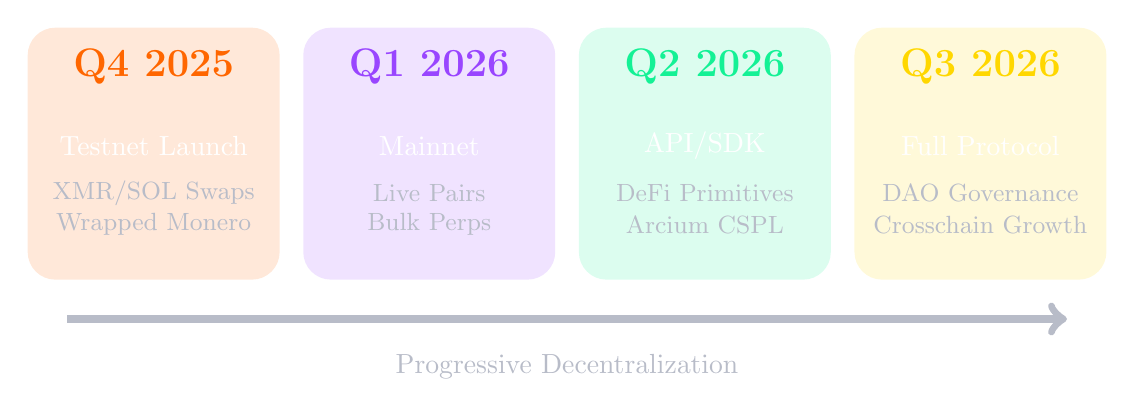
\begin{tikzpicture}
    % Q4 2025
    \fill[primary,opacity=0.15,rounded corners=10pt] (-7.5,2.8) rectangle (-4.3,6.0);
    \node[text=primary,font=\Large\bfseries] at (-5.9,5.5) {Q4 2025};
    \node[text=textprimary,font=\normalsize,align=center] at (-5.9,4.5) {Testnet Launch};
    \node[text=textsecondary,font=\small,align=center] at (-5.9,3.9) {XMR/SOL Swaps};
    \node[text=textsecondary,font=\small,align=center] at (-5.9,3.5) {Wrapped Monero};
    
    % Q1 2026
    \fill[secondary,opacity=0.15,rounded corners=10pt] (-4,2.8) rectangle (-0.8,6.0);
    \node[text=secondary,font=\Large\bfseries] at (-2.4,5.5) {Q1 2026};
    \node[text=textprimary,font=\normalsize,align=center] at (-2.4,4.5) {Mainnet};
    \node[text=textsecondary,font=\small,align=center] at (-2.4,3.9) {Live Pairs};
    \node[text=textsecondary,font=\small,align=center] at (-2.4,3.5) {Bulk Perps};
    
    % Q2 2026
    \fill[accent,opacity=0.15,rounded corners=10pt] (-0.5,2.8) rectangle (2.7,6.0);
    \node[text=accent,font=\Large\bfseries] at (1.1,5.5) {Q2 2026};
    \node[text=textprimary,font=\normalsize,align=center] at (1.1,4.5) {API/SDK};
    \node[text=textsecondary,font=\small,align=center] at (1.1,3.9) {DeFi Primitives};
    \node[text=textsecondary,font=\small,align=center] at (1.1,3.5) {Arcium CSPL};
    
    % Q3 2026
    \fill[highlight,opacity=0.15,rounded corners=10pt] (3,2.8) rectangle (6.2,6.0);
    \node[text=highlight,font=\Large\bfseries] at (4.6,5.5) {Q3 2026};
    \node[text=textprimary,font=\normalsize,align=center] at (4.6,4.5) {Full Protocol};
    \node[text=textsecondary,font=\small,align=center] at (4.6,3.9) {DAO Governance};
    \node[text=textsecondary,font=\small,align=center] at (4.6,3.5) {Crosschain Growth};
    
    % Timeline arrow
    \draw[->,line width=3pt,textsecondary] (-7,2.3) -- (5.7,2.3);
    \node[text=textsecondary,font=\normalsize] at (-0.65,1.7) {Progressive Decentralization};
  \end{tikzpicture}
\end{frame}

% -------------------------------------------------
\begin{frame}[t]{\color{textprimary}\textbf{Fun Gerbil: Cypherpunk Founders}}
  \begin{tikzpicture}[remember picture,overlay]
    \fill[primary,opacity=0.05] (current page.south west) rectangle (current page.north east);
  \end{tikzpicture}
  
  \centering
  \vspace{-0.5em}
  
  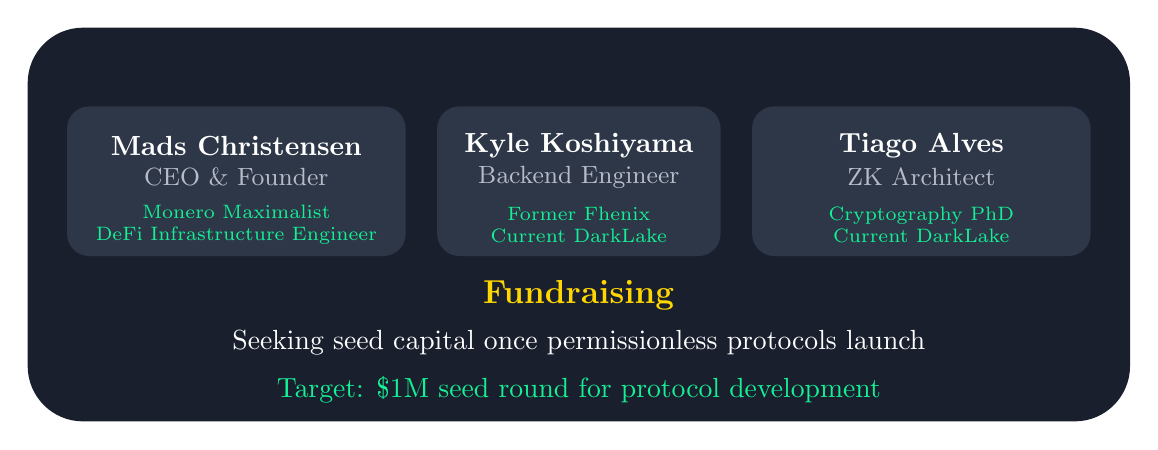
\begin{tikzpicture}
    % Team display moved up more
    \fill[midbg,rounded corners=20pt] (-7,-1.5) rectangle (7,3.5);
    

    
    % Team member boxes - better sizing with increased vertical space
    \fill[lightbg,rounded corners=8pt] (-6.5,0.6) rectangle (-2.2,2.5);
    \node[text=textprimary,font=\bfseries,align=center] at (-4.35,2.0) {Mads Christensen};
    \node[text=textsecondary,font=\small,align=center] at (-4.35,1.6) {CEO \& Founder};
    \node[text=accent,font=\scriptsize,align=center] at (-4.35,1.0) {Monero Maximalist \\ DeFi Infrastructure Engineer};
    
    \fill[lightbg,rounded corners=8pt] (-1.8,0.6) rectangle (1.8,2.5);
    \node[text=textprimary,font=\bfseries,align=center] at (0,2.0) {Kyle Koshiyama};
    \node[text=textsecondary,font=\small,align=center] at (0,1.6) {Backend Engineer};
    \node[text=accent,font=\scriptsize,align=center] at (0,1.0) {Former Fhenix\\Current DarkLake};
    
    \fill[lightbg,rounded corners=8pt] (2.2,0.6) rectangle (6.5,2.5);
    \node[text=textprimary,font=\bfseries,align=center] at (4.35,2.0) {Tiago Alves};
    \node[text=textsecondary,font=\small,align=center] at (4.35,1.6) {ZK Architect};
    \node[text=accent,font=\scriptsize,align=center] at (4.35,1.0) {Cryptography PhD\\Current DarkLake};
    
    % Backing info
    \node[text=highlight,font=\large,align=center] at (0,0.1) {\textbf{Fundraising}};
    \node[text=textprimary,font=\normalsize,align=center] at (0,-0.5) {Seeking seed capital once permissionless protocols launch};
    \node[text=accent,font=\normalsize,align=center] at (0,-1.1) {Target: \$1M seed round for protocol development};
  \end{tikzpicture}
\end{frame}

% -------------------------------------------------
\begin{frame}
  \begin{tikzpicture}[remember picture,overlay]
    \fill[primary,opacity=0.05] (current page.south west) rectangle (current page.north east);
    \fill[secondary,opacity=0.1] ([yshift=4cm]current page.south west) -- 
          (current page.south east) -- 
          (current page.north east) -- cycle;
  \end{tikzpicture}
  
  \centering
  \vspace{1em}
  
  {\fontsize{42}{50}\selectfont\color{textprimary}\textbf{Join the}}\\
  {\fontsize{52}{60}\selectfont\color{highlight}\textbf{PRIVACY}}\\
  {\fontsize{42}{50}\selectfont\color{textprimary}\textbf{Revolution}}
  
  \vspace{1.8em}
  
\begin{tikzpicture}
    \node[text=secondary,font=\Large] at (0,1.2) {\faGithub \quad github.com/madschristensen99/fungerbil};
    \node[text=primary,font=\Large] at (0,0.4) {\faTelegram \quad t.me/fungerbilswap};
    \node[text=accent,font=\Large] at (0,-0.4) {\faGlobe \quad fungerbil.com};
    
  \end{tikzpicture}
  
\end{frame}

\end{document}

